% siminos/CLE/Hilbert.tex

\subsection{Hilbert basis approach}

The most common approach to symmetry reduction is through the
use of a Hilbert basis of invariant polynomials. One computes
a (non-unique) basis of linearly independent polynomials,
invariant under the action of the symmetry group (\cf
\refref{gatermannHab,ChossLaut00} for a discussion of
methods) and either rewrites the dynamics in this basis or
maps the solutions to the polynomials.
The reader is referred to the book of Gilmore and
Lettelier\rf{GL-Gil07b} for a very detailed discussion of
symmetry reduction, through the use of invariant polynomials\ES{Also Chossat and Lauterbach?}.

For CLe it will be convenient to rewrite the action of $\Sigma=\SOn{2}$ acting on $\Rls{5}$ by
\beq
	x \mapsto  \Rot{\theta}x\,,
	\label{eq:SO2act}
\eeq
where
\beq
	\Rot{\theta}=	\left(\barr{ccccc}
				\cos(\theta) & -\sin(\theta) & 0	   & 0		    & 0\\
				\sin(\theta) & \cos(\theta)  & 0	   & 0		    & 0\\		
				0	     & 	0	     & \cos(\theta) & -\sin(\theta) & 0\\
				0	     &  0	     & \sin(\theta) & \cos(\theta) & 0\\
				0	     &  0	     & 0	    & 0		   & 1\\	
			\earr\right)\,,\ \ \theta\in[0,2\pi)\,.
    \label{eq:RotCLe5d}
\eeq


For the action \refeq{eq:SO2act} of
$\SOn{2}$ on \Rls{5} a Hilbert basis\rf{GL-Gil07b}  is
\beq
\begin{split}
	u_1 &= x_1^2+x_2^2 \cont
	u_2 &= y_1^2+y_2^2 \cont
	u_3 &= x_1 y_2-x_2 y_1\cont
	u_4 &= x_1 y_1+x_2 y_2\cont
	u_5 &= z\,.
	\label{eq:ipLaser}
\end{split}
\eeq
The polynomials in a Hilbert basis are linearly independent,
but often functionally dependent through relations called
\emph{syzygies}. For polynomials \refeq{eq:ipLaser} the
syzygy is
\beq
 	u_1u_2 -u_3^2-u_4^2 =0\,.
	\label{eq:syzLaser}
\eeq

%%%%%%%%%%%%%%%%%%%%%%%%%%%%%%%%%%%%%%%%%%%%%%%%%%%%%%%%%%%%%%%%%%
\begin{figure}[ht]
\begin{center}
  (\textit{a})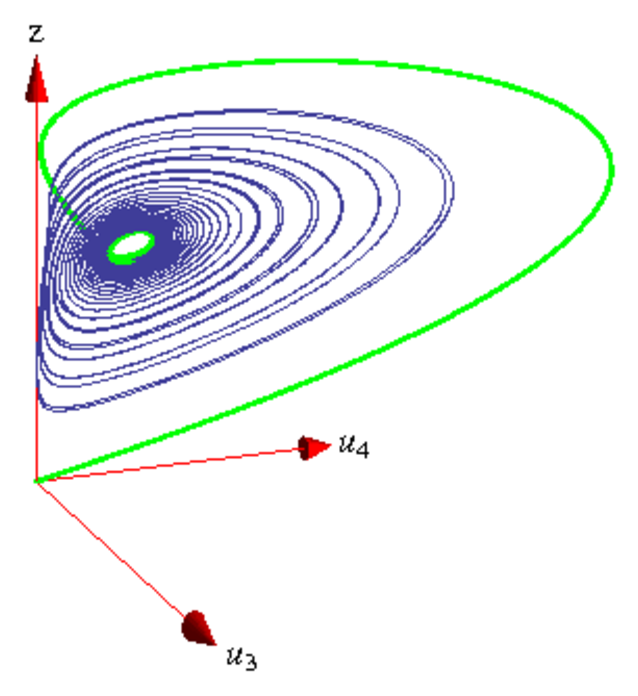
\includegraphics[width=0.35\textwidth]{../figs/CLEip1}
~~~~(\textit{b})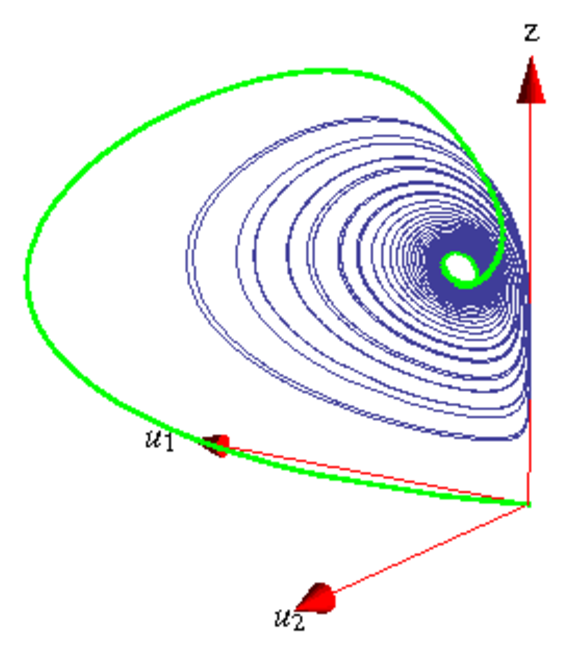
\includegraphics[width=0.36\textwidth]{../figs/CLEip2}
\end{center}
\caption[Orbit space projection of Complex Lorenz flow:
Invariant polynomials basis]{ \Statesp\ portraits of \CLe\
dynamics for $e=1/10$, $\ImrCLor=0$ in \reducedsp,
invariant polynomials basis \refeq{eq:ipLaser}.
    }
\label{fig:CLEip}
\end{figure}
%%%%%%%%%%%%%%%%%%%%%%%%%%%%%%%%%%%%%%%%%%%%%%%%%%%%%%%%%%%%%%%%

The first approach we try is by use of invariant polynomials
\refeq{eq:ipLaser}, following Gilmore and
Letellier\rf{GL-Gil07b} who compute an invariant polynomials
basis for the same action of $\SOn{2}$ and use them for
symmetry reduction of a system conjugate to \CLe, with
$e=-\ImrCLor$.
We use the chain rule
\beq
 \dot{\overline{x}}_i=\frac{\partial \overline{x}_i}{\partial x_j}\dot{x}_j
 \,,
\ee{ChainRul}
and express the result in invariant polynomials:
    \ES{mathematica notebook:CLEtransfJac.nb
    {\bf PC:} Changed $z$ to $u_5$; have not checked the algebra}
\beq
\begin{split}
\dot{u}_1 &=2\,\sigma\,(u_3-u_1)\,,\\
\dot{u}_2 &=-2\,u_2 -2\,u_3\,(u_5-\rho_1 )\,,\\
\dot{u}_3 &=\sigma\,  u_2-(\sigma\,  -1)\,u_3-e\,u_4+u_1\,(\rho_1-u_5)\,,\\
\dot{u}_4 &=e\, u_3-(\sigma\, +1)\,u_4\,,\\
\dot{u}_5 &=u_3-b\, u_5\,.
\end{split}
\label{eq:CLEip}
\eeq
For visualization purposes, rather than \ESedit{integrating
\refeq{eq:CLEip}, we map solutions of \refeq{eq:CLe} to the
$u_i$'s}, \reffig{fig:CLEip}. In most projections the folding
mechanism is hidden from view since the dynamics is squeezed
near the $z$-axis.

Nevertheless we can now easily identify a suitable Poincar\'e
section, guided by the Lorenz equations example,
    \PC{no such: ``
\refchap{chap:Lorenz},
    ''}
as one that contains the $z$-axis and
the \reqv, here defined by the condition $u_1=u_4$.
    \PC{no such: ``
Repeating
the procedure followed in \refsect{exmp:LorenzRetM}
    ''}
We
construct the first return map using as coordinate the
Euclidean length along the intersection of the unstable
manifold of \REQV{}{1} with the Poincar\'e surface of section,
measured from \REQV{}{1}, see \reffig{fig:CLEipRM}.


%%%%%%%%%%%%%%%%%%%%%%%%%%%%%%%%%%%%%%%%%%%%%%%%%%%%%%%%%%%%%%%%%%
\begin{figure}[ht]
\begin{center}
%   (\textit{a})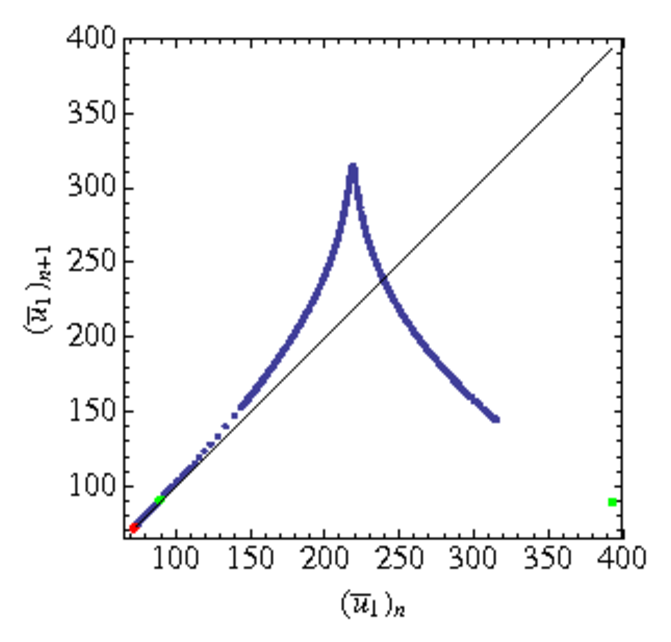
\includegraphics[width=0.35\textwidth]{../figs/CLEipRMu1}
%  ~~~~(\textit{b})
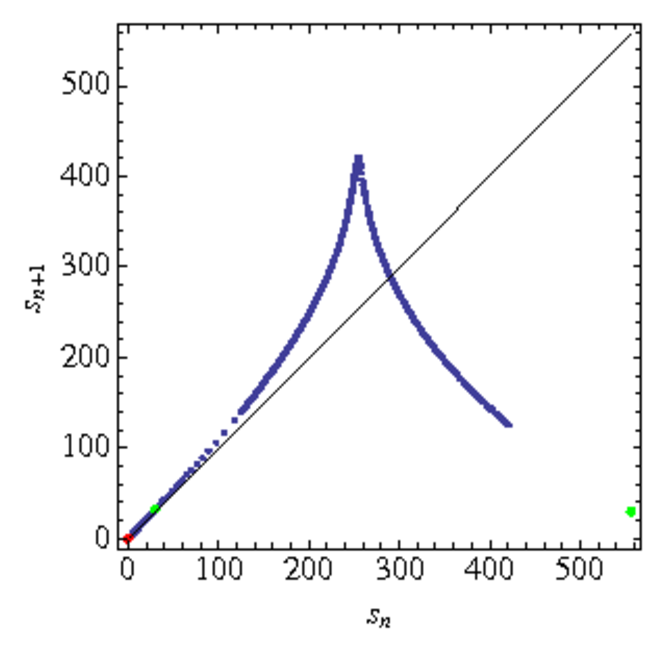
\includegraphics[width=0.35\textwidth]{../figs/CLEipRM}
\end{center}
\caption[Return map for Complex Lorenz flow, invariant polynomials]
{Return map to the \Poincare\
surface of section $u_1=u_4$ for \CLe\ with $e=1/10$, $\ImrCLor=0$,
projected on invariant polynomials \refeq{eq:ipLaser}.
% (a) The return map coordinate is $u_1$, (b)
The return map coordinate is the Euclidean
length along the \Poincare\ section of the unstable manifold of $E_1$.
    }
\label{fig:CLEipRM}
\end{figure}
%%%%%%%%%%%%%%%%%%%%%%%%%%%%%%%%%%%%%%%%%%%%%%%%%%%%%%%%%%%%%%%%


When one takes syzygies into account in rewriting the
dynamical system, singularities are introduced. Moreover when
one \emph{lifts} the dynamics from the quotient space
$\Manif/G$ to the original space $\Manif$ the transformations
have singularities at the \fixedsp s of
the isotropy subgroups in $\Manif$, in the optimal case, \cf
\refref{GL-Gil07b}. Those singularities do not seem to
restrict our ability to use invariant polynomials to obtain
symmetry reduced projections of the dynamics.
    \ES{define: \fixedsp}
    \PC{no such: ``
 as we will see in \refchap{chap:lasers}.
    ''}

What restricts the utility of Hilbert basis methods is that the
determination of a Hilbert basis becomes computationally
prohibitive as the dimension of the system or of the group
increases\rf{gatermannHab,ChossLaut00} and typically
computations are constrained to dimension smaller than ten. As
our goal is to quotient continuous symmetries of
high-dimensional flows, specifically those arising from
truncations of the \KS\ and Navier-Stokes flows
and thus we need an efficient framework.




